%-*-latex-*-
\sectionthree{Delete and extract-root}
\begin{python0}
  from solutions import *; clear()
\end{python0}

Suppose I want to delete
\texttt{8}
from this maxheap:


\begin{center}

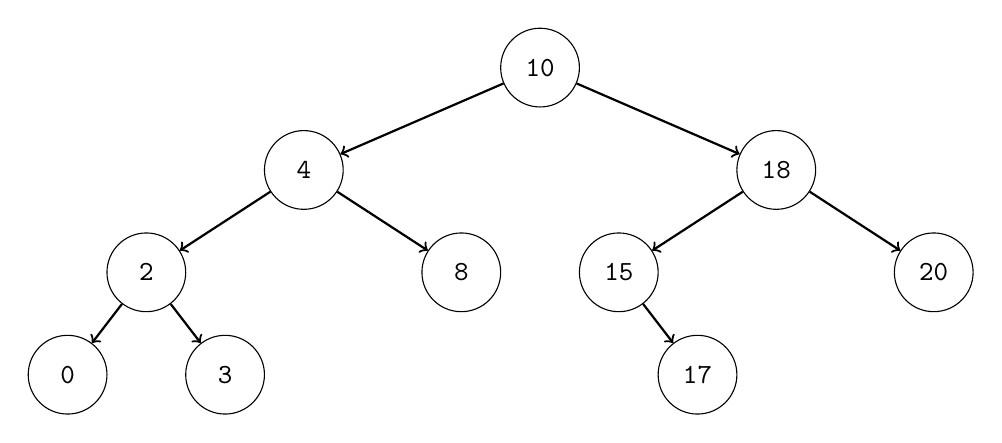
\begin{tikzpicture}
\node at (6,-1.3) [circle,draw,minimum size=10mm] (a) {\texttt{10}};
\node at (3,-2.6) [circle,draw,minimum size=10mm] (b) {\texttt{4}};
\node at (9,-2.6) [circle,draw,minimum size=10mm] (d) {\texttt{18}};
\node at (1,-3.9000000000000004) [circle,draw,minimum size=10mm] (e) {\texttt{2}};
\node at (5,-3.9000000000000004) [circle,draw,minimum size=10mm] (f) {\texttt{8}};
\node at (7,-3.9000000000000004) [circle,draw,minimum size=10mm] (h) {\texttt{15}};
\node at (11,-3.9000000000000004) [circle,draw,minimum size=10mm] (j) {\texttt{20}};
\node at (0,-5.2) [circle,draw,minimum size=10mm] (k) {\texttt{0}};
\node at (2,-5.2) [circle,draw,minimum size=10mm] (l) {\texttt{3}};
\node at (8,-5.2) [circle,draw,minimum size=10mm] (m) {\texttt{17}};
\draw [->,thick] (a) -- (b);
\draw [->,thick] (a) -- (d);
\draw [->,thick] (b) -- (e);
\draw [->,thick] (b) -- (f);
\draw [->,thick] (d) -- (h);
\draw [->,thick] (d) -- (j);
\draw [->,thick] (e) -- (k);
\draw [->,thick] (e) -- (l);
\draw [->,thick] (h) -- (m);

;
\end{tikzpicture}
    
\end{center}


from latextool_basic import *
p = Plot()
edges={20: [10, 8],
10: [ 9, 1],
8: [ 0, 7],
9: [ 2, 5],
}
drawheap(p, edges, include_array=False)
print(p)

In other words I want to delete the value at index 2
in the array implementation of the above heap.

I'll do it this way:
I look for the rightmost node of the last level --
this corresponds to the last value in the array implementation.
In the above case, that's the value \texttt{5}.
I then overwrite \texttt{8} with \texttt{5}:

from latextool_basic import *
print(automata(layout="""
   D  E  F
""",
edges="D,$a$,D|D,$b$,E|E,$b$,F|F,$a$,D",
D='initial|accept|label=$q_3$',
E='label=$q_4$',
F='label=$q_5$',
))

from latextool_basic import *
p = Plot()
edges={20: [10, 8],
10: [ 9, 1],
8: [ 0, 7],
9: [ 2, 5],
}
drawheap(p, edges, include_array=False)
p += Line(names=[5, 8], linewidth=0.03, endstyle='>', linecolor='red')
print(p)

to get this:


\begin{center}
\begin{tikzpicture}[>=triangle 60,shorten >=0.5pt,node distance=2cm,auto,initial text=, double distance=2pt]
\node[state] (A) at (  0,  0) {$a$};
\node[state] (B) at (  3,  0) {$b$};
\node[state] (F) at (  6,  0) {$f$};
\node[state] (C) at (  0, -2) {$c$};
\node[state] (D) at (  3, -2) {$d$};
\node[state] (E) at (  6, -2) {$e$};

\path[->]
(A) edge [loop above] node {} ()
(A) edge [bend left=0,pos=0.5,above] node {} (B)
(B) edge [bend left=0,pos=0.5] node {} (D)
(B) edge [bend left=0,pos=0.5,above] node {} (E)
(C) edge [bend left=0,pos=0.5,above] node {} (B)
(C) edge [bend left=0,pos=0.5,above] node {} (D)
(D) edge [bend left=0,pos=0.5,above] node {} (E)

;
\end{tikzpicture}
\end{center}
    

from latextool_basic import *
p = Plot()
edges={20: [10, 5],
10: [ 9, 1],
5: [ 0, 7],
9: [ 2],
}
drawheap(p, edges, include_array=False)
print(p)

Now this is not a maxheap. Do you see why?

I look at the children of \texttt{5}: \texttt{0} and \texttt{7}.
I swap \texttt{5} with the max of the children which is \texttt{7}

\begin{center}
\begin{tikzpicture}
\draw[line width=0.03cm,red,<->] (5) to [bend left=60]  (7);

\fill[blue!10] (0.0, 0.0) circle (0.35);
\node [line width=0.03cm,black,minimum size=0.6699999999999999cm,draw,circle] at (0.0,0.0)(20){};\draw (0.0, 0.0) node[color=black] {\texttt{20}};
\fill[blue!10] (-1.9, -1.0) circle (0.35);
\node [line width=0.03cm,black,minimum size=0.6699999999999999cm,draw,circle] at (-1.9,-1.0)(10){};\draw (-1.9, -1.0) node[color=black] {\texttt{10}};
\fill[blue!10] (1.9, -1.0) circle (0.35);
\node [line width=0.03cm,black,minimum size=0.6699999999999999cm,draw,circle] at (1.9,-1.0)(5){};\draw (1.9, -1.0) node[color=black] {\texttt{5}};
\fill[blue!10] (-2.85, -2.0) circle (0.35);
\node [line width=0.03cm,black,minimum size=0.6699999999999999cm,draw,circle] at (-2.85,-2.0)(9){};\draw (-2.85, -2.0) node[color=black] {\texttt{9}};
\fill[blue!10] (-0.95, -2.0) circle (0.35);
\node [line width=0.03cm,black,minimum size=0.6699999999999999cm,draw,circle] at (-0.95,-2.0)(1){};\draw (-0.95, -2.0) node[color=black] {\texttt{1}};
\fill[blue!10] (0.95, -2.0) circle (0.35);
\node [line width=0.03cm,black,minimum size=0.6699999999999999cm,draw,circle] at (0.95,-2.0)(0){};\draw (0.95, -2.0) node[color=black] {\texttt{0}};
\fill[blue!10] (2.85, -2.0) circle (0.35);
\node [line width=0.03cm,black,minimum size=0.6699999999999999cm,draw,circle] at (2.85,-2.0)(7){};\draw (2.85, -2.0) node[color=black] {\texttt{7}};
\fill[blue!10] (-3.33, -3.0) circle (0.35);
\node [line width=0.03cm,black,minimum size=0.6699999999999999cm,draw,circle] at (-3.33,-3.0)(2){};\draw (-3.33, -3.0) node[color=black] {\texttt{2}};\draw[line width=0.03cm,black] (20) to  (10);
\draw[line width=0.03cm,black] (20) to  (5);
\draw[line width=0.03cm,black] (10) to  (9);
\draw[line width=0.03cm,black] (10) to  (1);
\draw[line width=0.03cm,black] (5) to  (0);
\draw[line width=0.03cm,black] (5) to  (7);
\draw[line width=0.03cm,black] (9) to  (2);
\end{tikzpicture}

\end{center}


from latextool_basic import *
p = Plot()
edges={20: [10, 5],
10: [ 9, 1],
5: [ 0, 7],
9: [ 2],
}
p += Line(names=[5, 7], linewidth=0.03, endstyle='>',
startstyle='>', linecolor='red', bend_left=60)
drawheap(p, edges, include_array=False)
print(p)

and get this:

\begin{center}
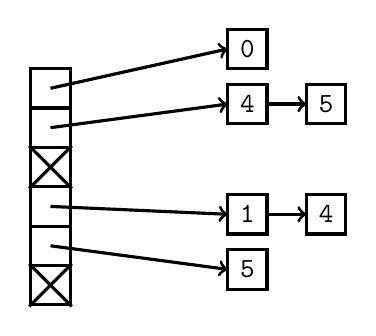
\begin{tikzpicture}

\draw (0.25, -0.25)
  node[draw, line width=0.04cm, , color=black,
       rounded corners=0cm, inner sep=0cm] {

\begin{minipage}[t][0.5cm]{0.5cm}
\mbox{}

\end{minipage}

};
\draw (0.25, -0.75)
  node[draw, line width=0.04cm, , color=black,
       rounded corners=0cm, inner sep=0cm] {

\begin{minipage}[t][0.5cm]{0.5cm}
\mbox{}

\end{minipage}

};
\draw (0.25, -1.25)
  node[draw, line width=0.04cm, , color=black,
       rounded corners=0cm, inner sep=0cm] {

\begin{minipage}[t][0.5cm]{0.5cm}
\mbox{}

\end{minipage}

};
\draw (0.25, -1.75)
  node[draw, line width=0.04cm, , color=black,
       rounded corners=0cm, inner sep=0cm] {

\begin{minipage}[t][0.5cm]{0.5cm}
\mbox{}

\end{minipage}

};
\draw (0.25, -2.25)
  node[draw, line width=0.04cm, , color=black,
       rounded corners=0cm, inner sep=0cm] {

\begin{minipage}[t][0.5cm]{0.5cm}
\mbox{}

\end{minipage}

};
\draw (0.25, -2.75)
  node[draw, line width=0.04cm, , color=black,
       rounded corners=0cm, inner sep=0cm] {

\begin{minipage}[t][0.5cm]{0.5cm}
\mbox{}

\end{minipage}

};\draw[line width=0.04cm,black] (-0.02,-0.98) to  (0.52,-1.52);
\draw[line width=0.04cm,black] (0.52,-0.98) to  (-0.02,-1.52);
\draw[line width=0.04cm,black] (-0.02,-2.48) to  (0.52,-3.02);
\draw[line width=0.04cm,black] (0.52,-2.48) to  (-0.02,-3.02);

\draw (2.75, 0.24999999999999992)
  node[draw, line width=0.04cm, , color=black,
       rounded corners=0cm, inner sep=0cm] {

\begin{minipage}[t][0.5cm]{0.5cm}
\mbox{}

\end{minipage}

};\draw (2.75, 0.24999999999999992) node[color=black] {{\texttt{0}}};
\draw (2.75, -0.45000000000000007)
  node[draw, line width=0.04cm, , color=black,
       rounded corners=0cm, inner sep=0cm] {

\begin{minipage}[t][0.5cm]{0.5cm}
\mbox{}

\end{minipage}

};\draw (2.75, -0.45000000000000007) node[color=black] {{\texttt{4}}};
\draw (3.75, -0.45000000000000007)
  node[draw, line width=0.04cm, , color=black,
       rounded corners=0cm, inner sep=0cm] {

\begin{minipage}[t][0.5cm]{0.5cm}
\mbox{}

\end{minipage}

};\draw (3.75, -0.45000000000000007) node[color=black] {{\texttt{5}}};
\draw (2.75, -1.85)
  node[draw, line width=0.04cm, , color=black,
       rounded corners=0cm, inner sep=0cm] {

\begin{minipage}[t][0.5cm]{0.5cm}
\mbox{}

\end{minipage}

};\draw (2.75, -1.85) node[color=black] {{\texttt{1}}};
\draw (3.75, -1.85)
  node[draw, line width=0.04cm, , color=black,
       rounded corners=0cm, inner sep=0cm] {

\begin{minipage}[t][0.5cm]{0.5cm}
\mbox{}

\end{minipage}

};\draw (3.75, -1.85) node[color=black] {{\texttt{4}}};
\draw (2.75, -2.55)
  node[draw, line width=0.04cm, , color=black,
       rounded corners=0cm, inner sep=0cm] {

\begin{minipage}[t][0.5cm]{0.5cm}
\mbox{}

\end{minipage}

};\draw (2.75, -2.55) node[color=black] {{\texttt{5}}};\draw[line width=0.04cm,black,->] (0.25,-0.25) to  (2.5,0.25);
\draw[line width=0.04cm,black,->] (0.25,-0.75) to  (2.5,-0.45);
\draw[line width=0.04cm,black,->] (3.0,-0.45) to  (3.5,-0.45);
\draw[line width=0.04cm,black,->] (0.25,-1.75) to  (2.5,-1.85);
\draw[line width=0.04cm,black,->] (3.0,-1.85) to  (3.5,-1.85);
\draw[line width=0.04cm,black,->] (0.25,-2.25) to  (2.5,-2.55);
\end{tikzpicture}

\end{center}


from latextool_basic import *
p = Plot()
edges={20: [10, 7],
10: [ 9, 1],
7: [ 0, 5],
9: [ 2],
}
drawheap(p, edges, include_array=False)
print(p)

Clearly, we keep pushing \texttt{5} down as much as possible until
we get a maxheap again (i.e., heapify-down).
It might take more than one swap.

This above method works as long as \texttt{5} is a descendent of the
value to be removed.

Usually the value to be delete is in fact the root of the heap.
When the root is to be deleted, then the operation is called
\defone{extract-max} for the case of maxheap
and \defone{extract-min} for the case of
minheap.
I'm going to call both of them \defone{extract-root}.

Let's do another example.
Let's delete \texttt{20} (the root) from this maxheap:

from latextool_basic import *
print(automata(layout="""
   D  E  F

      C1 D1
   A1 
      G1
""",
edges="D,$a$,D|D,$b$,E|E,$b$,F|F,$a$,D|A1,$b$,C1|C1,$a$,D1|D1,$b$,A1|A1,$a$,G1|G1,$b$,A1|D,$\ep$,A1",
D='initial|label=$q_3$',
E='label=$q_4$',
F='label=$q_5$',
A1='accept|label=$q_7$',
C1='label=$q_9$',
D1='label=$q_{10}$',
G1='label=$q_{13}$',
))

from latextool_basic import *
p = Plot()
edges={20: [10, 8],
10: [ 9, 1],
8: [ 0, 7],
9: [ 2, 5],
}
drawheap(p, edges, include_array=False)
print(p)


Again, I overwrite \texttt{20} with \texttt{5}

\begin{center}
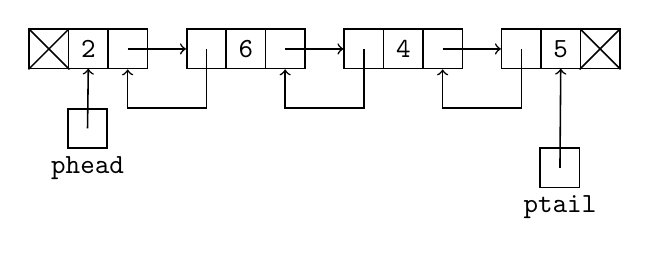
\begin{tikzpicture}

\draw (0.25, 0.25)
  node[draw, line width=0.02cm, , color=black,
       rounded corners=0cm, inner sep=0cm] {

\begin{minipage}[t][0.5cm]{0.5cm}
\mbox{}

\end{minipage}

};\draw (0.25, 0.25) node[color=black] {{\texttt{}}};
\draw (0.75, 0.25)
  node[draw, line width=0.02cm, , color=black,
       rounded corners=0cm, inner sep=0cm] {

\begin{minipage}[t][0.5cm]{0.5cm}
\mbox{}

\end{minipage}

};\draw (0.75, 0.25) node[color=black] {{\texttt{2}}};
\draw (1.25, 0.25)
  node[draw, line width=0.02cm, , color=black,
       rounded corners=0cm, inner sep=0cm] {

\begin{minipage}[t][0.5cm]{0.5cm}
\mbox{}

\end{minipage}

};\draw (1.25, 0.25) node[color=black] {{\texttt{}}};
\draw (2.25, 0.25)
  node[draw, line width=0.02cm, , color=black,
       rounded corners=0cm, inner sep=0cm] {

\begin{minipage}[t][0.5cm]{0.5cm}
\mbox{}

\end{minipage}

};\draw (2.25, 0.25) node[color=black] {{\texttt{}}};
\draw (2.75, 0.25)
  node[draw, line width=0.02cm, , color=black,
       rounded corners=0cm, inner sep=0cm] {

\begin{minipage}[t][0.5cm]{0.5cm}
\mbox{}

\end{minipage}

};\draw (2.75, 0.25) node[color=black] {{\texttt{6}}};
\draw (3.25, 0.25)
  node[draw, line width=0.02cm, , color=black,
       rounded corners=0cm, inner sep=0cm] {

\begin{minipage}[t][0.5cm]{0.5cm}
\mbox{}

\end{minipage}

};\draw (3.25, 0.25) node[color=black] {{\texttt{}}};
\draw (4.25, 0.25)
  node[draw, line width=0.02cm, , color=black,
       rounded corners=0cm, inner sep=0cm] {

\begin{minipage}[t][0.5cm]{0.5cm}
\mbox{}

\end{minipage}

};\draw (4.25, 0.25) node[color=black] {{\texttt{}}};
\draw (4.75, 0.25)
  node[draw, line width=0.02cm, , color=black,
       rounded corners=0cm, inner sep=0cm] {

\begin{minipage}[t][0.5cm]{0.5cm}
\mbox{}

\end{minipage}

};\draw (4.75, 0.25) node[color=black] {{\texttt{4}}};
\draw (5.25, 0.25)
  node[draw, line width=0.02cm, , color=black,
       rounded corners=0cm, inner sep=0cm] {

\begin{minipage}[t][0.5cm]{0.5cm}
\mbox{}

\end{minipage}

};\draw (5.25, 0.25) node[color=black] {{\texttt{}}};
\draw (6.25, 0.25)
  node[draw, line width=0.02cm, , color=black,
       rounded corners=0cm, inner sep=0cm] {

\begin{minipage}[t][0.5cm]{0.5cm}
\mbox{}

\end{minipage}

};\draw (6.25, 0.25) node[color=black] {{\texttt{}}};
\draw (6.75, 0.25)
  node[draw, line width=0.02cm, , color=black,
       rounded corners=0cm, inner sep=0cm] {

\begin{minipage}[t][0.5cm]{0.5cm}
\mbox{}

\end{minipage}

};\draw (6.75, 0.25) node[color=black] {{\texttt{5}}};
\draw (7.25, 0.25)
  node[draw, line width=0.02cm, , color=black,
       rounded corners=0cm, inner sep=0cm] {

\begin{minipage}[t][0.5cm]{0.5cm}
\mbox{}

\end{minipage}

};\draw (7.25, 0.25) node[color=black] {{\texttt{}}};\draw[line width=0.02cm,black,->] (1.25,0.25) to  (1.99,0.25);
\draw[line width=0.02cm,black,->] (3.25,0.25) to  (3.99,0.25);
\draw[line width=0.02cm,black,->] (2.25,0.25) to  (2.25,-0.5) to  (1.25,-0.5) to  (1.25,-0.01);
\draw[line width=0.02cm,black,->] (5.25,0.25) to  (5.99,0.25);
\draw[line width=0.02cm,black,->] (4.25,0.25) to  (4.25,-0.5) to  (3.25,-0.5) to  (3.25,-0.01);
\draw[line width=0.02cm,black,->] (6.25,0.25) to  (6.25,-0.5) to  (5.25,-0.5) to  (5.25,-0.01);
\draw[line width=0.02cm,black] (-0.01,0.51) to  (0.51,-0.01);
\draw[line width=0.02cm,black] (0.51,0.51) to  (-0.01,-0.01);
\draw[line width=0.02cm,black] (6.99,0.51) to  (7.51,-0.01);
\draw[line width=0.02cm,black] (7.51,0.51) to  (6.99,-0.01);

\draw (0.74, -0.76)
  node[draw, line width=0.02cm, , color=black,
       rounded corners=0cm, inner sep=0cm] {

\begin{minipage}[t][0.5cm]{0.5cm}
\mbox{}

\end{minipage}

};\draw (0.74, -0.76) node[color=black] {{\texttt{}}};
\draw (0.74, -1.26)
  node[draw, line width=0.02cm, , color=white,
       rounded corners=0cm, inner sep=0cm] {

\begin{minipage}[t][0.1cm]{0.1cm}
\mbox{}

\end{minipage}

};\draw (0.74, -1.26) node[color=black] {{\texttt{phead}}};\draw[line width=0.02cm,black,->] (0.74,-0.76) to  (0.75,0);

\draw (6.74, -1.26)
  node[draw, line width=0.02cm, , color=black,
       rounded corners=0cm, inner sep=0cm] {

\begin{minipage}[t][0.5cm]{0.5cm}
\mbox{}

\end{minipage}

};\draw (6.74, -1.26) node[color=black] {{\texttt{}}};
\draw (6.74, -1.76)
  node[draw, line width=0.02cm, , color=white,
       rounded corners=0cm, inner sep=0cm] {

\begin{minipage}[t][0.1cm]{0.1cm}
\mbox{}

\end{minipage}

};\draw (6.74, -1.76) node[color=black] {{\texttt{ptail}}};\draw[line width=0.02cm,black,->] (6.74,-1.26) to  (6.75,0);
\end{tikzpicture}

\end{center}


from latextool_basic import *
p = Plot()
edges={'20': [10, 8],
10: [ 9, 1],
8: [ 0, 7],
9: [ 2, '5'],
}
drawheap(p, edges, include_array=False)
p += Line(names=['5', '20'], linecolor='red', endstyle='>', linewidth=0.03)      
print(p)

(\texttt{5} is chosen, again because it's the rightmost
in the last level, or equivalently, it's the last in the
corresponding array implementation.)
I get this:

\begin{center}
\begin{tikzpicture}

\fill[white] (19.0, -0.6) circle (0.3);
\node [line width=0.03cm,black,minimum size=0.57cm,draw,circle] at (19.0,-0.6)(A){};\draw (19.0, -0.6) node[color=black] {\texttt{20}};
\fill[white] (16.0, -1.0) circle (0.3);
\node [line width=0.03cm,black,minimum size=0.57cm,draw,circle] at (16.0,-1.0)(a){};\draw (16.0, -1.0) node[color=black] {\texttt{10}};
\fill[white] (10.0, -2.0) circle (0.3);
\node [line width=0.03cm,black,minimum size=0.57cm,draw,circle] at (10.0,-2.0)(b){};\draw (10.0, -2.0) node[color=black] {\texttt{0}};
\fill[white] (11.0, -4.0) circle (0.3);
\node [line width=0.03cm,black,minimum size=0.57cm,draw,circle] at (11.0,-4.0)(d){};\draw (11.0, -4.0) node[color=black] {\texttt{18}};
\fill[white] (8.0, -3.0) circle (0.3);
\node [line width=0.03cm,black,minimum size=0.57cm,draw,circle] at (8.0,-3.0)(e){};\draw (8.0, -3.0) node[color=black] {\texttt{-2}};
\fill[white] (7.0, -4.0) circle (0.3);
\node [line width=0.03cm,black,minimum size=0.57cm,draw,circle] at (7.0,-4.0)(k){};\draw (7.0, -4.0) node[color=black] {\texttt{-3}};
\fill[white] (9.0, -4.0) circle (0.3);
\node [line width=0.03cm,black,minimum size=0.57cm,draw,circle] at (9.0,-4.0)(l){};\draw (9.0, -4.0) node[color=black] {\texttt{-1}};
\fill[white] (15.0, -4.0) circle (0.3);
\node [line width=0.03cm,black,minimum size=0.57cm,draw,circle] at (15.0,-4.0)(h){};\draw (15.0, -4.0) node[color=black] {\texttt{8}};
\fill[white] (14.0, -5.0) circle (0.3);
\node [line width=0.03cm,black,minimum size=0.57cm,draw,circle] at (14.0,-5.0)(m){};\draw (14.0, -5.0) node[color=black] {\texttt{6}};
\fill[white] (13.0, -3.0) circle (0.3);
\node [line width=0.03cm,black,minimum size=0.57cm,draw,circle] at (13.0,-3.0)(f){};\draw (13.0, -3.0) node[color=black] {\texttt{5}};
\fill[white] (13.0, -6.0) circle (0.3);
\node [line width=0.03cm,black,minimum size=0.57cm,draw,circle] at (13.0,-6.0)(n){};\draw (13.0, -6.0) node[color=black] {\texttt{4}};
\fill[white] (15.0, -6.0) circle (0.3);
\node [line width=0.03cm,black,minimum size=0.57cm,draw,circle] at (15.0,-6.0)(o){};\draw (15.0, -6.0) node[color=black] {\texttt{7}};
\fill[white] (18.0, -2.0) circle (0.3);
\node [line width=0.03cm,black,minimum size=0.57cm,draw,circle] at (18.0,-2.0)(p){};\draw (18.0, -2.0) node[color=black] {\texttt{15}};\draw[line width=0.03cm,black,->,>=triangle 60] (A) to  (a);
\draw[line width=0.03cm,black,->,>=triangle 60] (a) to  (p);
\draw[line width=0.03cm,black,->,>=triangle 60] (a) to  (b);
\draw[line width=0.03cm,black,->,>=triangle 60] (b) to  (e);
\draw[line width=0.03cm,black,->,>=triangle 60] (b) to  (f);
\draw[line width=0.03cm,black,->,>=triangle 60] (f) to  (d);
\draw[line width=0.03cm,black,->,>=triangle 60] (f) to  (h);
\draw[line width=0.03cm,black,->,>=triangle 60] (e) to  (k);
\draw[line width=0.03cm,black,->,>=triangle 60] (e) to  (l);
\draw[line width=0.03cm,black,->,>=triangle 60] (h) to  (m);
\draw[line width=0.03cm,black,->,>=triangle 60] (m) to  (n);
\draw[line width=0.03cm,black,->,>=triangle 60] (m) to  (o);
\end{tikzpicture}

\end{center}


from latextool_basic import *
p = Plot()
edges={5: [10, 8],
10: [ 9, 1],
8: [ 0, 7],
9: [ 2],
}
drawheap(p, edges, include_array=False)
print(p)

I do the same again as above: I pick the larger of the children
of \texttt{5}, which in this case is \texttt{10} and swap with \texttt{5}.
I get this:

\begin{center}
\begin{tikzpicture}

\fill[white] (19.0, -0.6) circle (0.3);
\node [line width=0.03cm,black,minimum size=0.57cm,draw,circle] at (19.0,-0.6)(A){};\draw (19.0, -0.6) node[color=black] {\texttt{20}};
\fill[white] (16.0, -1.0) circle (0.3);
\node [line width=0.03cm,black,minimum size=0.57cm,draw,circle] at (16.0,-1.0)(a){};\draw (16.0, -1.0) node[color=black] {\texttt{10}};\draw[line width=0.1cm,black] (15.8,-1.2) to  (16.2,-0.8);

\fill[white] (16.0, -2.0) circle (0.3);
\node [line width=0.03cm,white,minimum size=0.57cm,draw,circle] at (16.0,-2.0)(aa){};\draw (16.0, -2.0) node[color=black] {\texttt{8}};\draw[line width=0.05cm,black,->,>=triangle 60] (aa) to  (a);

\fill[white] (10.0, -2.0) circle (0.3);
\node [line width=0.03cm,black,minimum size=0.57cm,draw,circle] at (10.0,-2.0)(b){};\draw (10.0, -2.0) node[color=black] {\texttt{0}};
\fill[white] (11.0, -4.0) circle (0.3);
\node [line width=0.03cm,black,minimum size=0.57cm,draw,circle] at (11.0,-4.0)(d){};\draw (11.0, -4.0) node[color=black] {\texttt{18}};
\fill[white] (18.0, -2.0) circle (0.3);
\node [line width=0.03cm,black,minimum size=0.57cm,draw,circle] at (18.0,-2.0)(p){};\draw (18.0, -2.0) node[color=black] {\texttt{15}};
\fill[white] (8.0, -3.0) circle (0.3);
\node [line width=0.03cm,black,minimum size=0.57cm,draw,circle] at (8.0,-3.0)(e){};\draw (8.0, -3.0) node[color=black] {\texttt{-2}};
\fill[white] (7.0, -4.0) circle (0.3);
\node [line width=0.03cm,black,minimum size=0.57cm,draw,circle] at (7.0,-4.0)(k){};\draw (7.0, -4.0) node[color=black] {\texttt{-3}};
\fill[white] (9.0, -4.0) circle (0.3);
\node [line width=0.03cm,black,minimum size=0.57cm,draw,circle] at (9.0,-4.0)(l){};\draw (9.0, -4.0) node[color=black] {\texttt{-1}};
\fill[white] (15.0, -4.0) circle (0.3);
\node [line width=0.03cm,black,,dashed,minimum size=0.57cm,draw,circle] at (15.0,-4.0)(h){};\draw (15.0, -4.0) node[color=black] {\texttt{8}};
\fill[white] (14.0, -5.0) circle (0.3);
\node [line width=0.03cm,black,minimum size=0.57cm,draw,circle] at (14.0,-5.0)(m){};\draw (14.0, -5.0) node[color=black] {\texttt{6}};
\fill[white] (13.0, -3.0) circle (0.3);
\node [line width=0.03cm,black,minimum size=0.57cm,draw,circle] at (13.0,-3.0)(f){};\draw (13.0, -3.0) node[color=black] {\texttt{5}};
\fill[white] (13.0, -6.0) circle (0.3);
\node [line width=0.03cm,black,minimum size=0.57cm,draw,circle] at (13.0,-6.0)(n){};\draw (13.0, -6.0) node[color=black] {\texttt{4}};
\fill[white] (15.0, -6.0) circle (0.3);
\node [line width=0.03cm,black,minimum size=0.57cm,draw,circle] at (15.0,-6.0)(o){};\draw (15.0, -6.0) node[color=black] {\texttt{7}};\draw[line width=0.03cm,black,->,>=triangle 60] (A) to  (a);
\draw[line width=0.03cm,black,->,>=triangle 60] (a) to  (p);
\draw[line width=0.03cm,black,->,>=triangle 60] (a) to  (b);
\draw[line width=0.03cm,black,->,>=triangle 60] (b) to  (e);
\draw[line width=0.03cm,black,->,>=triangle 60] (b) to  (f);
\draw[line width=0.03cm,black,->,>=triangle 60] (f) to  (d);
\draw[line width=0.03cm,black,->,>=triangle 60] (e) to  (k);
\draw[line width=0.03cm,black,->,>=triangle 60] (e) to  (l);
\draw[line width=0.03cm,black,->,>=triangle 60] (m) to  (n);
\draw[line width=0.03cm,black,->,>=triangle 60] (m) to  (o);
\draw[line width=0.03cm,black,->,>=triangle 60,dashed] (f) to  (h);
\draw[line width=0.03cm,black,->,>=triangle 60,dashed] (h) to  (m);
\draw[line width=0.07cm,black,->,>=triangle 60] (f) to  (m);
\end{tikzpicture}

\end{center}


from latextool_basic import *
p = Plot()
edges={10: [ 5, 8],
5: [ 9, 1],
8: [ 0, 7],
9: [ 2],
}
drawheap(p, edges, include_array=False)
print(p)

It's not a maxheap yet.
I look at the children of \texttt{5} and choose the largest,
which would be \texttt{9}, and swap it with \texttt{5}.
Here's what I get:

\begin{center}
\begin{tikzpicture}

\fill[white] (0.0, 0.0) circle (0.4);
\node [line width=0.03cm,black,minimum size=0.77cm,draw,circle] at (0.0,0.0)(1){};\draw (0.0, 0.0) node[color=black] {$q_5$};
\fill[white] (5.0, 0.0) circle (0.4);
\node [line width=0.03cm,black,minimum size=0.77cm,draw,circle] at (5.0,0.0)(2){};\draw (5.0, 0.0) node[color=black] {$q_2$};\draw[line width=0.03cm,black,->,>=triangle 60] (1) to node [above] {$\ep, \ep \rightarrow \ep $} (2);
\end{tikzpicture}

\end{center}


from latextool_basic import *
p = Plot()
edges={10: [ 9, 8],
9: [ 5, 1],
8: [ 0, 7],
5: [ 2],
}
drawheap(p, edges, include_array=False)
print(p)

Ahhh ... at this point I have a maxheap.
I'm done!

\begin{console}[commandchars=\\\{\}]
  ALGORITHM: heap_delete (for maxheap)
  INPUT: x - an array representing a maxheap
  n - the length of the heap in x (pass by reference)
  i - index of value to be removed (note usually
  this is 0)

  x[i] = x[n - 1]
  n = n - 1
  heapify_down(x, i)
\end{console}

(Note that because of the shape of the tree -- a complete tree --
a node cannot have a right child but no left child.)

Recall what I just said: usually the delete operation for maxheap
occurs at index 0, i.e., you're removing the maximum value in the maxheap.
In that case the operation is also called extract-max or delete-max.
You'll see why when we use this delete operation to perform heapsort
and when we use this for priority queues.

Note that the runtime is
\[
  O(\log n)
\]
since the heapify-down operation basically moves
a value in the tree down to the leaf level, possibly stopping
early.
This means that the worse runtime must be
the height of the tree which is $O(\log n)$.

\newpage
\begin{ex}
  You are given this maxheap:

  \begin{center}
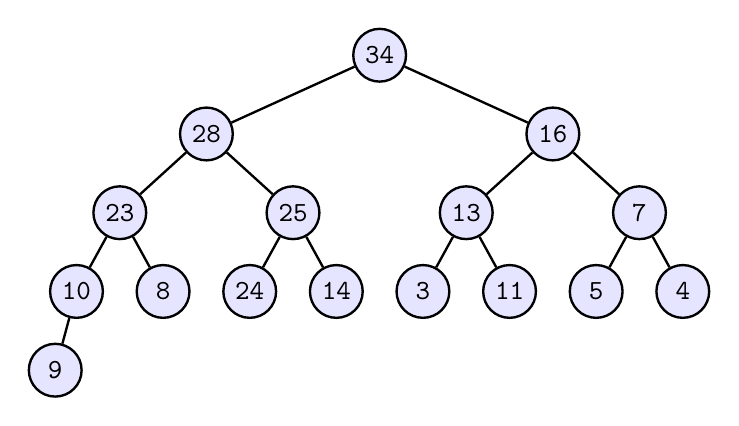
\begin{tikzpicture}

\fill[blue!10] (0.0, 0.0) circle (0.35);
\node [line width=0.03cm,black,minimum size=0.6699999999999999cm,draw,circle] at (0.0,0.0)(34){};\draw (0.0, 0.0) node[color=black] {\texttt{34}};
\fill[blue!10] (-2.2, -1.0) circle (0.35);
\node [line width=0.03cm,black,minimum size=0.6699999999999999cm,draw,circle] at (-2.2,-1.0)(28){};\draw (-2.2, -1.0) node[color=black] {\texttt{28}};
\fill[blue!10] (2.2, -1.0) circle (0.35);
\node [line width=0.03cm,black,minimum size=0.6699999999999999cm,draw,circle] at (2.2,-1.0)(16){};\draw (2.2, -1.0) node[color=black] {\texttt{16}};
\fill[blue!10] (-3.3, -2.0) circle (0.35);
\node [line width=0.03cm,black,minimum size=0.6699999999999999cm,draw,circle] at (-3.3,-2.0)(23){};\draw (-3.3, -2.0) node[color=black] {\texttt{23}};
\fill[blue!10] (-1.1, -2.0) circle (0.35);
\node [line width=0.03cm,black,minimum size=0.6699999999999999cm,draw,circle] at (-1.1,-2.0)(25){};\draw (-1.1, -2.0) node[color=black] {\texttt{25}};
\fill[blue!10] (1.1, -2.0) circle (0.35);
\node [line width=0.03cm,black,minimum size=0.6699999999999999cm,draw,circle] at (1.1,-2.0)(13){};\draw (1.1, -2.0) node[color=black] {\texttt{13}};
\fill[blue!10] (3.3, -2.0) circle (0.35);
\node [line width=0.03cm,black,minimum size=0.6699999999999999cm,draw,circle] at (3.3,-2.0)(7){};\draw (3.3, -2.0) node[color=black] {\texttt{7}};
\fill[blue!10] (-3.85, -3.0) circle (0.35);
\node [line width=0.03cm,black,minimum size=0.6699999999999999cm,draw,circle] at (-3.85,-3.0)(10){};\draw (-3.85, -3.0) node[color=black] {\texttt{10}};
\fill[blue!10] (-2.75, -3.0) circle (0.35);
\node [line width=0.03cm,black,minimum size=0.6699999999999999cm,draw,circle] at (-2.75,-3.0)(8){};\draw (-2.75, -3.0) node[color=black] {\texttt{8}};
\fill[blue!10] (-1.65, -3.0) circle (0.35);
\node [line width=0.03cm,black,minimum size=0.6699999999999999cm,draw,circle] at (-1.65,-3.0)(24){};\draw (-1.65, -3.0) node[color=black] {\texttt{24}};
\fill[blue!10] (-0.55, -3.0) circle (0.35);
\node [line width=0.03cm,black,minimum size=0.6699999999999999cm,draw,circle] at (-0.55,-3.0)(14){};\draw (-0.55, -3.0) node[color=black] {\texttt{14}};
\fill[blue!10] (0.55, -3.0) circle (0.35);
\node [line width=0.03cm,black,minimum size=0.6699999999999999cm,draw,circle] at (0.55,-3.0)(3){};\draw (0.55, -3.0) node[color=black] {\texttt{3}};
\fill[blue!10] (1.65, -3.0) circle (0.35);
\node [line width=0.03cm,black,minimum size=0.6699999999999999cm,draw,circle] at (1.65,-3.0)(11){};\draw (1.65, -3.0) node[color=black] {\texttt{11}};
\fill[blue!10] (2.75, -3.0) circle (0.35);
\node [line width=0.03cm,black,minimum size=0.6699999999999999cm,draw,circle] at (2.75,-3.0)(5){};\draw (2.75, -3.0) node[color=black] {\texttt{5}};
\fill[blue!10] (3.85, -3.0) circle (0.35);
\node [line width=0.03cm,black,minimum size=0.6699999999999999cm,draw,circle] at (3.85,-3.0)(4){};\draw (3.85, -3.0) node[color=black] {\texttt{4}};
\fill[blue!10] (-4.12, -4.0) circle (0.35);
\node [line width=0.03cm,black,minimum size=0.6699999999999999cm,draw,circle] at (-4.12,-4.0)(9){};\draw (-4.12, -4.0) node[color=black] {\texttt{9}};\draw[line width=0.03cm,black] (34) to  (28);
\draw[line width=0.03cm,black] (34) to  (16);
\draw[line width=0.03cm,black] (28) to  (23);
\draw[line width=0.03cm,black] (28) to  (25);
\draw[line width=0.03cm,black] (16) to  (13);
\draw[line width=0.03cm,black] (16) to  (7);
\draw[line width=0.03cm,black] (23) to  (10);
\draw[line width=0.03cm,black] (23) to  (8);
\draw[line width=0.03cm,black] (25) to  (24);
\draw[line width=0.03cm,black] (25) to  (14);
\draw[line width=0.03cm,black] (13) to  (3);
\draw[line width=0.03cm,black] (13) to  (11);
\draw[line width=0.03cm,black] (7) to  (5);
\draw[line width=0.03cm,black] (7) to  (4);
\draw[line width=0.03cm,black] (10) to  (9);
\end{tikzpicture}

\end{center}


  from latextool_basic import *
  p = Plot()
  edges={'34':['28','16'],
  '28':['23','25'],
  '16':['13','7'],
  '23':['10','8'],
  '25':['24','14'],
  '13':['3','11'],
  '7':['5','4'],
  '10':['9'],
  }
  drawheap(p, edges, node_hsep=0.2,
  include_array=False)
  print(p)

  Do the following operations one after another,
  drawing the tree including the swaps
  and the final
  maxheap.
  Also, draw the corresponding array.
  \begin{tightlist}
  \item Delete \texttt{28}.
  \item Delete \texttt{34}
  \item Delete \texttt{16}
  \item Delete the maximum value in the maxheap, i.e., perform extract max.
  \item Delete the maximum value in the maxheap, i.e., perform extract max.
  \end{tightlist}
\end{ex}

\newpage
\begin{ex}
  Draw a minheap with 15 distinct values.
  Extract the minimum and draw the minheap.
  Do it again.
  \qed
\end{ex}





\begin{ex}
  Using an array, 
  build a maxheap by inserting the following into an empty tree:
  1, 3, 5, 7, 6, 4, 2, 0, 8, 9.
  Make sure the tree is complete after each insert and the leaves
  at the lowest level are all on the left.
  Call the array \texttt{x}
  (assume it has size at least 10)
  and use integer variable \texttt{len}
  for the length of \texttt{x}.
  Of course initially \texttt{len} is 0.
  \qed
\end{ex}

\begin{ex}
  Using the maxheap (using an array) from the previous question,
  remove the following values one after another left to right:
  \[
    1, 3, 5, 7, 6, 4, 2, 0, 8, 9
  \]
  Call the array \texttt{x} and use integer variable \texttt{len}
  for the length of \texttt{x}.
  Of course initially \texttt{len} is 10.
  Make sure that after each delete, the tree is complete after each delete and 
  the leaves
  at the lowest level are all on the left.
  \qed
\end{ex}

\begin{ex}
  Suppose during an extract-root for minheap,
  you need to heapify-down at an index \verb!i!.
  Suppose the left and right child value of \verb!x[i]! are the same and
  larger than \verb!x[i]!.
  Which do you prefer to swap with \verb!x[i]!, the left or the right
  child?
\end{ex}
% choose the right because the tree might be one step shorter on the right
% and therefore the heapify down might terminate earlier by 1 step
%
% Example:
%     5
%    1 1
%   3

\begin{ex}
  Suppose you have a heap whose array is \verb!x!.
  In this heap, if you extract the root and you insert the same value back
  into the heap, will the heap be the same as the original \verb!x!?
  \qed
\end{ex}
%NO
%    1
%  2   3
%
%    2
%  3
%
%    2      --->      1
%  3   1            3   2
%
